\chapter{Introducción}

Los objetos compactos (también llamados estrellas compactas) son el residuo de la vida luminosa de las estrellas, llamados así porque su tamaño es significativamente más pequeño que el de una estrella normal/en la secuencia principal con una masa similar, estos objetos pueden alcanzar densidades superiores a la densidad de saturación nuclear  ($\rho_0=\num{2.3e+14}\,\si{g/cm^3}$) y a las que los potenciales gravitacionales son tan grandes que la relatividad general es importante para determinar su estructura (exceptuando a las enanas blancas). \REMARK{Quizá sea bueno introducir la clasificación de una}

Como remanentes de estrellas, vale la pena discutir a grandes rasgos el proceso de formación y evolución estelar antes de estudiar a mayor profundidad la estructura de los objetos compactos, ya que permitirá tener una idea general de los procesos que llevan a una estrella a su destino final.   \TODO{Pulir justificación} 

\section{Resumen de evolución estelar}
Las estrellas son formadas a partir de nubes de gas interestelar, compuestas en su mayoría de hidrógeno molecular, que debido a algún tipo de perturbación (como una onda de choque) comienzan a colapsar sobre ellas mismas gravitacionalmente. La energía gravitacional es convertida en calor por la contracción y si la temperatura incrementa lo suficiente ($T \approx 10^7 \, \si{\kelvin}$, punto de ignición para la fusión de hidrógeno a helio), con ayuda de la contracción adicional causada por la pérdida de energía por radiación, la fusión se convierte en la fuente de energía principal y la presión termal y de radiación balancearán la gravedad, permitiendo así que la estrella se forme \cite{Glendenning2000CompactStars}.

Las reacciones nucleares pueden sostener la estrella por un gran periodo de tiempo (de millones a billones de años, dependiendo de la masa de la estrella) en lo que se conoce como su fase de secuencia principal, llamada así porque las estrellas en esta etapa forman una secuencia mono-paramétrica (ignorando la composición química), cuyo parámetro es la masa estelar, en el diagrama de Hertzsprung-Russell (ver Figura \ref{HR}).
Las estrellas pasan la mayor parte de su vida luminosa en este estado, razón por la cual la mayoría de estrellas son encontradas en la secuencia principal, hasta que después de un tiempo característico el hidrógeno es extinguido/consumido/usado casi en su totalidad dejando un núcleo de Helio y da inicio a una siguiente etapa de fusión, de Helio a Carbono, el proceso se repite a lo largo de varias etapas de combustión (carbono, neón, oxígeno, magnesio y silicio) \cite{Scilla2016IntroductionEvolution}. \TODO{Revisar el orden del ciclo y por qué algunos elementos se saltan}

\begin{figure}[H]
    \centering
    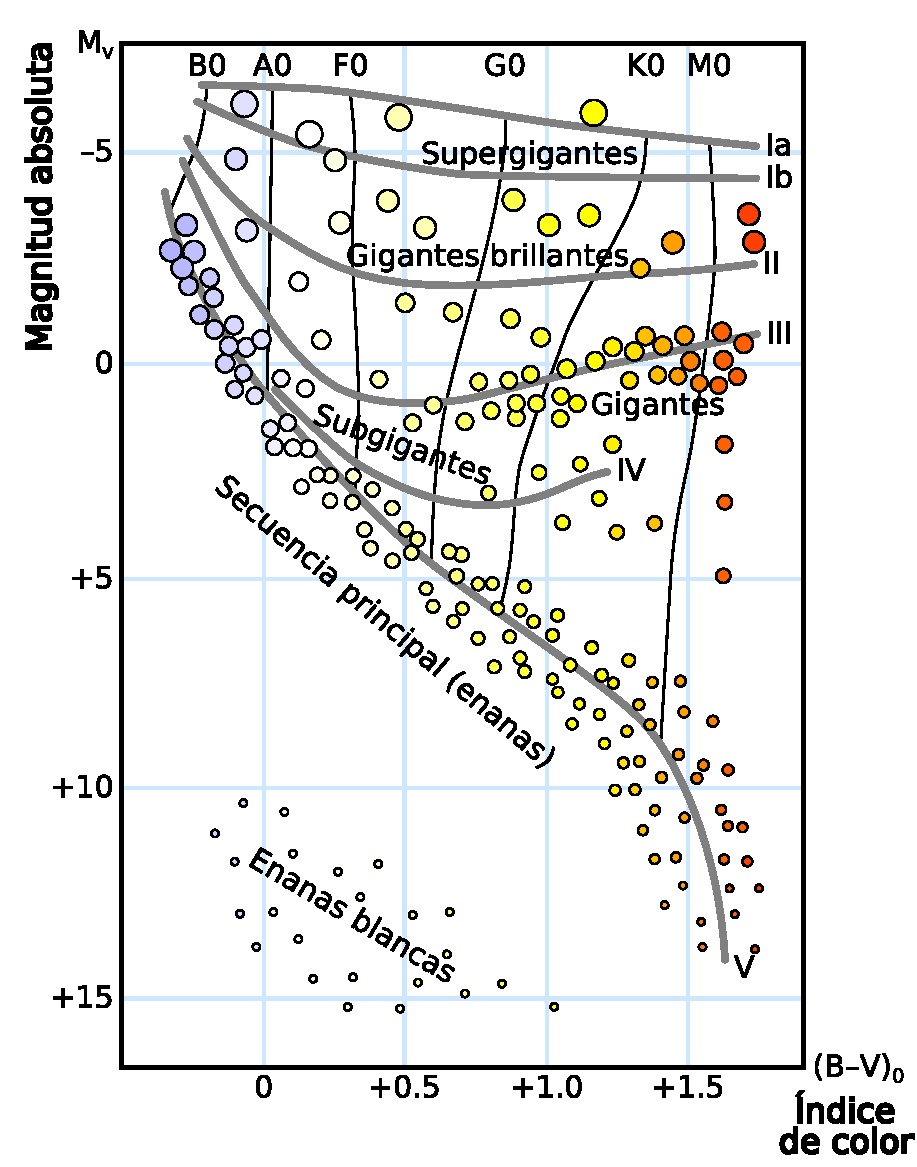
\includegraphics[width=250pt]{figures/H-R_diagram.pdf}%
    \caption{Diagrama Hertzsprung-Russell}
    \label{HR}
\end{figure}

%\begin{multicols}{2}[\columnsep2em] 

%\columnbreak
%\end{multicols}  
%y resultarán, después de un evento complejo y violento, como una estrella de neutrones o un agujero negro. \REMARK{No he hablado ni de estrellas de neutrones ni de agujeros negros...} 


El ciclo de combustión termina al alcanzar el hierro, debido a que la energía de enlace por nucleón tiene su valor máximo para el hierro y la fusión deja de ser exotérmica. Qué tanto avanza una estrella en este ciclo dependerá de la masa estelar, sólo estrellas masivas ($M \geq 8 M_{\odot} $) llegan al hierro/final, en este punto tendrán una estructura en forma de cascarones de materia que rodean al núcleo de hierro. Sin la energía producida por la fusión nuclear la compresión de la gravedad no tiene qué la equipare y la estrella colapsa, las capas de materia caen casi libremente hacia el núcleo desencadenando, a través de mecanismos complejos y no enteramente comprendidos, una supernova de colapso de núcleo \cite{Woosley2005TheSupernovae} \cite{Janka2012ExplosionSupernovae}.

El núcleo colapsado o proto-objeto compacto inicia un proceso de enfriamiento y reajustamiento estructural hasta que alcanza su composición de equilibrio de neutrones, protones, hiperones, leptones y posiblemente quarks, altamente degenerados, es decir, en un estado tal que han ocupado los niveles de energía más bajos disponibles. El objeto compacto formado será sostenido por la presión de degeneración de las partículas degeneradas que lo compongan \cite{Glendenning2000CompactStars}. Vale la pena aclarar que se acostumbra llamar a todos estos objetos estrellas de neutrones, aunque su composición puede ser tan variada como se mencionó antes.     
\TODO{Ya que se sabe qué es un objeto compacto, hablar a grandes rasgos de la estructura global de estos y la dependencia de la ecuación de estado, para darle paso a mi problema.}
\TODO{Papers seminales en estructura global y algunos de ecuaciones de estado.}
